\documentclass[a4paper,draft]{report}

\usepackage{fontspec}
\setmonofont[Scale=0.8]{DejaVu Sans Mono}

\usepackage{fullpage}
\usepackage{unicode-math}
\usepackage{amsmath}
\usepackage{mathtools}
\usepackage{hyperref}  % ref
\usepackage{color}
\usepackage{booktabs}  % nice tables
\usepackage{float}
\usepackage{acronym}


%% Code
\usepackage{catchfilebetweentags}
\usepackage{agda/latex/agda}

\usepackage{minted}
\usepackage{fancyvrb}
\usemintedstyle{default}

\newmint{haskell}{mathescape,fontfamily=tt}
\newmintedfile{haskell}{mathescape,fontfamily=tt}
\newminted{haskell}{gobble=8,mathescape,fontfamily=tt}
\newmint{coq}{mathescape,fontfamily=tt}
\newmintedfile{coq}{mathescape,fontfamily=tt}
\newminted{coq}{gobble=8,mathescape,fontfamily=tt}



%% Metainformation
%% PDF stuff
\usepackage{datetime}
\usepackage{ifpdf}
\ifpdf
\pdfinfo{
    /Author (João Paulo Pizani Flor)
    /Title (PiWare: An Embedded Hardware Description Language using Dependent Types)
    /Keywords (EDSL, HDL, Hardware Description, Functional Programming, Dependent types, Agda, Coq, Lava, Coquet)
    /CreationDate (D:\pdfdate)
}
\fi

\title{Π-Ware: An Embedded Hardware Description Language using Dependent Types}

\date{\today}

\author{
    João Paulo Pizani Flor \\
    Department of Information and Computing Sciences, \\
    Utrecht University - The Netherlands \\
    e-mail: j.p.pizaniflor@students.uu.nl
}



%% The document itself
\begin{document}

    \maketitle


    \chapter{Introduction}
    \label{chap:intro}
        Several factors have been causing an increasing demand for hardware acceleration of algorithms,
        and there is also pressure to reduce the duration and cost of the circuit design process.
        These trends collide with the techniques and tooling used in the hardware design process,
        which have not experienced the same evolution as the ones for software development.

        \acrodef{ASIC}{Application-Specific Integrated Circuit}
        The design of an \ac{ASIC} imposes strong requirements,
        specially with regards to correctness (functional and otherwise).
        Design mistakes which make their way into the manufacturing process can be very expensive,
        and errors that reach the consumer even more, as there's no such thing as "updating" a chip.
        One infamous example of such a bug reaching the consumer was the \emph{FDIV} bug in Intel's Pentium chip,
        which might have costed the company over 400 million dollars~\cite{intel-fdiv}.

        In the software industry, and specially
        in application domains requiring high correctness assurance (such as information security, machine control, etc.),
        functional programming techniques have long been used to improve productivity
        and reduce the need for extensive testing and debugging.
        Advocates of functional programming claim productivity gains of up to 10 times to
        programmers coming from an imperative environment.

        Another advantage usually attributed to functional programming is an increased capacity to
        \emph{reason} about your programs, specially to perform what is called \emph{equational reasoning}.
        These claims have been confirmed in practice (and still keep getting more confirmations),
        and furthermore, functional techniques and constructs keep "penetrating" imperative languages
        with each new release. For example, the SWIFT language, released by Apple in 2014,
        includes features such as immutable data structures, first-class functions and type inference.

        % TODO: Purely functional programming examples

        In a certain way, we can compare the power of the tools and techniques
        used nowadays in hardware design to the early days of software development.
        % TODO: Simulation languages were "shoehorned" into hardware description.
        Of course there are inherent and fundamental differences between the two activities, but
        this comparison leads us to ask whether ideas from programming language research,
        specially those related to functional programming, could be used to improve hardware design.

        \acrodef{EDSL}{Embedded Domain-Specific Language}
        Research trying to answer this broad question started already in the 1980s,
        with the work of Prof. Mary Sheeran and others~\cite{sheeran-survey},
        developing \emph{functional} hardware description languages, such as \emph{μFP}.
        Later, a trend emerged of developing \acp{EDSL} for hardware description,
        \emph{hosted} in functional languages, such as Haskell.
        % TODO: Lava, ForSyDe, etc. ALREADY KINDA PRACTICALLY VALIDATED AND USED

        \acrodef{DTP}{Dependently-Typed Programming}
        Staying on the "path" of functional programming but going even further in power we reach \ac{DTP}.
        A type system with \emph{dependent types} can express very powerful properties about the programs written in it.
        In fact, a dependent type can express any formula of \emph{intuitionistic first-order logic} and,
        according to the \emph{Curry-Howard correspondence},
        inhabitants of a type correspond to proofs of the logical statement represented by the type.

        Therefore, using dependent types, one can more easily approximate \emph{specification} and \emph{implementation}.
        The type signature of a function can give much more \emph{guarantees} about its behaviour.
        We can have, for example, the type of a "vector grouping" function as follows:

        \begin{listing}[h]
            \ExecuteMetaData[agda/latex/Report/Chapter1.tex]{group-decl}
            \caption{Signature of a vector grouping function, with dependent types. \label{lst:group-decl}}
        \end{listing}

        The return type of this function reads as:
        \begin{quote}
            There is a vector \texttt{xss} of size \texttt{n}
            (whose elements are of size \texttt{k}), such that \texttt{concat xss ≡ xs}.
        \end{quote}

        Therefore, it returns a collection of groups "sliced" from the original vector, with the requested size.
        Additionally, it returns a proof that concatenating the groups results in the original vector.
        This type serves as a \emph{specification of correctness} for the function.
        Any function with this type is, by definition, a \emph{correct "grouping" function}.

        %% Only for deep-embedded
        In an \ac{EDSL} for hardware there will usually be a \emph{type} whose elements are circuits.
        One can imagine that it would be useful to design this type in such a way that as few of its elements as possible are \emph{malformed}.
        Therefore, we also want to make the typing of the circuits as strong as possible,
        to eliminate as many classes of design mistakes as possible.

        %% TODO: Tie up motivation here

        Depedent type systems allow us to easily express several of these \emph{well-formedness} rules for circuits.
        One simple criterion of circuit \emph{well-formedness} is, for example, that it contains no ``floating'' signals.
        That is, all of a circuit's internal components must have all their ports connected. % TODO: to something?

        \begin{figure}[h]
            \centerline{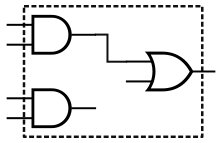
\includegraphics[width=0.5\textwidth]{imgs/floating-wire.pdf}}
            \caption{TODO: floating wire diagram \label{fig:floating-wire}}
        \end{figure}

        In this M.Sc thesis, we developed a hardware \ac{EDSL} -- Π-Ware -- which enforces this and other
        well-formedness rules using dependent types.
        Π-Ware is a \emph{deep-embedded} \ac{EDSL} hosted in the Agda programming language,
        that supports synthesis to (VHDL) netlists and simulation for combinational and synchronous sequential circuits.
        Furthermore, the user of Π-Ware can prove \emph{expressive} properties about circuits in the logic
        of Agda itself (intuitionistic first-order logic).

        %% TODO: Summarize a bit

        \begin{itemize}
            \item Research question, methodology
            \begin{itemize}
                \item In which way can dependent types make circuit design a more precise and efficient activity?
                \item We develop an EDSL for hardware - Π-Ware - embedded in the DT language Agda
                \begin{itemize}
                    \item Characteristics of Π-Ware:
                    \begin{itemize}
                        \item Deep-embedded
                        \item Synthesis to netlists
                        \item Simulation semantics
                        \item Low AND high level of data abstraction
                        \item Prove STRONG properties (first-order logic) about circuit behaviour interactively
                    \end{itemize}
                \end{itemize}
            \end{itemize}
        \end{itemize}


    \chapter{Background}
    \label{chap:hardware}

        \section{Hardware Description}
        \label{sec:hardware-description}
            \begin{itemize}
                \item Compare software and hardware
                \item Target models of computation: register machine x boolean circuits
                    \subitem trade-off in complexity (size x cycles)

                \item General trend to raise the level of abstraction of descriptions
                \item Hardware description languages

                \item Attempts at High-Level Synthesis and so forth (TCC)
            \end{itemize}

            The hardware development process can be well understood by analyzing its
            similarities and differences to software development.
            Both hardware and software development usually "begins" with a high-level \emph{specification}
            of the algorithm to be implemented.
            Also, both proceed by a series of transformations, increasingly adding more details to the description.

            However, the final targets of both hardware and software development differ:
            while in software the final artifact is machine code (sequence of instructions) for some architecture,
            in hardware the target is usually a \emph{floorplan}, a spacially placed graph of logic gates and wires.
            Also, the transformation steps in the software and hardware chains are different, as follows:

            \begin{figure}[h]
                \centerline{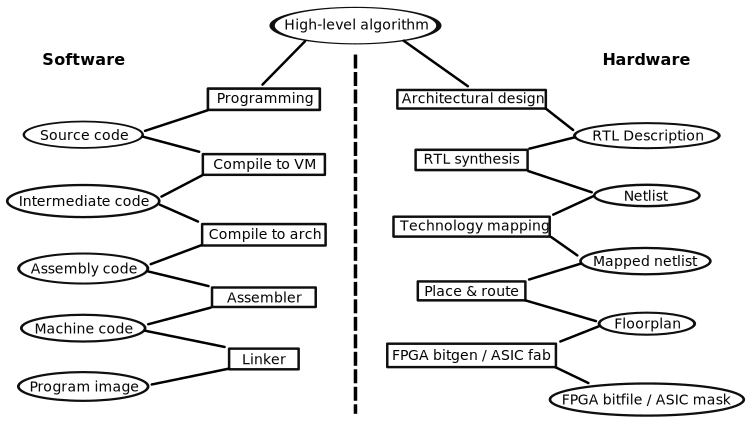
\includegraphics[width=0.5\textwidth]{imgs/sw-hw-chains.pdf}}
                \caption{TODO: Software and Hardware refinement chains \label{fig:sw-hw-chains}}
            \end{figure}

            \acrodef{HDL}{Hardware Description Language}
            \acrodef{RTL}{Register-Transfer Level}
            The first (higher) levels in this series of transformations is usually described using
            so-called \acp{HDL}, most popularly Verilog and VHDL.
            However, these languages were originally designed for \emph{simulation} purposes,
            and there are several problems that arise when using them to model hardware
            \emph{architecture} at \ac{RTL}.


        \section{Functional Hardware Description}
        \label{sec:functional-hardware}
            \begin{itemize}
                \item Embedded functional HDLs
                \item Lava, etc.
            \end{itemize}


        \section{Dependently-Typed Programming}
        \label{sec:dtp}

            \subsection{Dependent types}
            \label{subsec:dependent-types}
                \begin{itemize}
                    \item General type system explanation, growing in power until we reach dependent types
                    \item Expressivity of dependent types
                        \subitem Curry-Howard correspondence
                        \subitem Practical examples
                            \subsubitem Especially powerful for EDSLs (The Power of Pi)
                            \subsubitem Segway into circuit EDSLs
                \end{itemize}

                A type system, in the context of computer programming,
                serves the purpose of grouping values, so that "meaningless" and potentially undesirable operations are avoided.
                For example, it would be silly to add an integer number and a character string.
                In fact, it is hard to imagine an addition operation accepting such arguments and having nice algebraic properties.
                To define addition sensibly, therefore, we need the help of a type system, to "ban" all programs that would
                try to add these "incompatible" values.

                Type systems can have very different properties and be implemented in very different ways.
                Some of the ways in which type systems can be categorized are:
                \begin{itemize}
                    \item Weak vs. strong
                    \item Static vs. dynamic
                    \item Polymorphism (which form)
                    \item Etc.
                \end{itemize}
                %% TODO: cite old general types paper from the TPT seminar

                %% TODO: the "road to" dependent types
                The most basic form of abstraction -- values depending on values (the concept of functions) -- is
                supported in practically all type systems.
                Then there is values depending on types, polymorphism, where a can function can display different
                behaviour depending on the type of its input.
                Going one step further, some type systems support types that depend on other types, these are
                called \emph{type operators} or \emph{type-level functions}.

                \begin{figure}[h]
                    \centerline{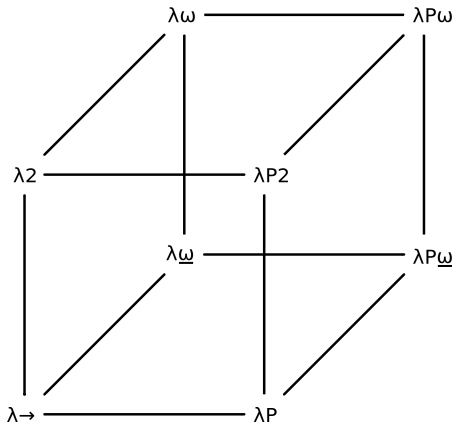
\includegraphics[width=0.5\textwidth]{imgs/lambda-cube.pdf}}
                    \caption{TODO: Barendregt's "Lambda Cube" \label{fig:lambda-cube}}
                \end{figure}

            \subsection{Hardware and dependent types}
            \label{sec:hardware-dtp}
                \begin{itemize}
                    \item Others
                    \item Coquet
                        \subitem Turning design mistakes into TYPE ERRORS
                        \subitem Proving properties about circuit behaviour
                        \subsubitem Functional correctness in particular.
                \end{itemize}


    \chapter{The Π-Ware library}
    \label{chap:piware}
        Lorem ipsum\ldots

        %% How to present:
            %% By design decisions ∨

        \section{Circuit Syntax}
        \label{sec:circuit-types}
            \begin{itemize}
                \item Shallow vs. deep embedding
                    \subitem Chose deep because of synthesis and non-functional analyses
                \item Structural modelling
                    \subitem Represent connections among circuits in the DSL, \emph{not in the metalanguage}
                    \subitem Avoid having to deal with observable sharing
            \end{itemize}

        \section{Abstraction Mechanisms}
        \label{sec:abstraction}
            \begin{itemize}
                \item Data abstraction (atom vectors x arbitrary synthesizable types)
                    \subitem Atom (enumeration axioms)
                    \subitem Word / Synthesizable
                        \subsubitem Proof search?
                \item Gate abstraction (Technology primitives x Semantic fundamentals)
                    \subitem Circuits descriptions are parameterized by a set of fundamental gates
                        \subsubitem Always combinational
                        \subsubitem Their correctness is assumed
                    \subitem For synthesis, still need to give these gates a description in terms of technology primitives
            \end{itemize}

        \section{Circuit Semantics}
        \label{sec:eval-seq}
            \begin{itemize}
                \item Two types of evaluation: combinational and sequential
                \item Combinational eval requires a proof that the circuit contains no loops
                    \subitem Eval of a fundamental gate is just its \emph{definitional behaviour}

                \item For sequential circuits we use a \emph{causal stream semantics}
                %% TODO: couldn't we restrict it even more and just keep ONE PAST VALUE in the context?
                    \subitem Current output depends on the current input and (possibly) on the past input
                    \subitem \emph{Different} than plain Stream functions

                \item There's also an eval function which allows the circuit to be viewed as function from Stream to Stream
            \end{itemize}


    \chapter{Conclusions}
    \label{chap:conclusions}
        \begin{itemize}
            \item Reiterate what was achieved
            \item Prioritize what still needs to be done, or would be nice if done
        \end{itemize}

        \section{Discussion and Related Work}
        \label{sec:related-work}
            Lorem ipsum\ldots

        \section{Future work}
        \label{sec:future-work}
            \begin{itemize}
                \item What problems \emph{Π-Ware} still has.
                    \subitem With suggestions for how to solve them, if possible

                \item More broadly, considering \emph{Π-Ware}, what would be the ``next steps''.
            \end{itemize}


    \newpage
    \bibliographystyle{plain}
    \bibliography{references}

\end{document}
